\documentclass[12pt]{article}
\usepackage[utf8]{inputenc}
\usepackage{graphicx}
\usepackage{amsmath}
\usepackage{caption}
\usepackage{subcaption}
\usepackage{listings}
\usepackage{float}
\usepackage{geometry}
\geometry{margin=1in}

\title{Analysis of Merge Sort and its Parallel Implementations}
\author{Mauti Enzo}
\date{\today}

\begin{document}

\maketitle

\begin{abstract}
This report contain a quick analysis of the merge sort algorithm, 2 parallelized implementation of the algorithm, one using OpenMP, the other using MPI.
We will then analyse the strong and weak scaling of each of the implementation and finish by presenting possible enhancement of those implementations.
\end{abstract}

\section{Introduction}
Merge Sort is a divide-and-conquer algorithm with a worst-case and average-case time complexity of \( O(n \log n) \).

\section{Sequential Merge Sort}

\subsection{Algorithm Description}
\noindent\fbox{
  \parbox{\textwidth}{
\ttfamily
void mergeSort(std::vector<int>\& arr, int left, int right)\\
\{\\
\hspace*{1em}if (left >= right)\\
\hspace*{2em}return;\\
\\
\hspace*{1em}int mid = left + (right - left) / 2;\\
\hspace*{1em}mergeSort(arr, left, mid);\\
\hspace*{1em}mergeSort(arr, mid + 1, right);\\
\hspace*{1em}merge(arr, left, mid, right);\\
\}
  }
}


\subsection{Complexity Analysis}
With \(T(k)\) as the time taken to sort \(k\) element and \(M(k)\) the time take to merge \(k\) element, we can write:

\begin{gather}
  T(N) = 2 \times T(\frac{N}{2}) + M(N) \\
  T(N) = 2 \times T(\frac{N}{2}) + constant \times N \\
  T(N) = 2^k \times T(\frac{N}{2^k}) + 2 \times N \times constant \\
  T(N) = N \times T(1) + N \times log_2N \times constant \\
  T(N) = N + N \times log_2N
\end{gather}

Therefore the time complexity is \textbf{\(O(N \times log_2N)\)}

\section{MPI Parallel Merge Sort}

\subsection{Algorithm Description}
\noindent\fbox{
  \parbox{\textwidth}{
\ttfamily
Initialize MPI

master process: \\
\hspace*{1em}create random vector 'arr' of size 'vector\_size'

compute 'counts' and 'displacements' for each rank \\
\hspace*{1em}scatter chunks of 'arr' to each process → 'local\_arr'

each process: \\
\hspace*{1em}sort its 'local\_arr' with mergeSort

gather all 'local\_arr' segments back to master

master process: \\
\hspace*{1em} for each segment received: \\
\hspace*{2em} merge in-place with previous segments

\hspace*{1em} check if final array is sorted \\
\hspace*{1em} print elapsed time \\
finalize MPI
  }
}

\subsection{Parallel Strategy}
In this implementation, we divide the array so that we can apply the sorting in multiple places at the same time.
The division is made based on the number of cores available at each time.
The transfert of datas is handled by the MPI functions \texttt{Scatterv} and \texttt{GatherV}.
Each subarray are then sorted, and sent back to the master process.
we then proceeds to a final merge among all subarrays.

\section{OpenMP Parallel Merge Sort}

\subsection{Algorithm Description}
\noindent\fbox{
  \parbox{\textwidth}{
\ttfamily
create random vector 'arr' of size 'vector\_size'

start OpenMP parallel region with 'num\_threads': \\
\hspace*{1em} single thread: \\
\hspace*{2em} call mergeSort(arr, 0, vector\_size - 1) \\
\hspace*{3em} recursively split into subtasks until size < THRESHOLD \\
\hspace*{3em} execute subtasks in parallel and merge in-place

check if final array is sorted

print elapsed time
  }
}


\subsection{Parallel Strategy}
In this implementation, we divide the workload between multiple threads, until a certain size threshold is achieved.
To accomplish that, we use the \texttt{\#pragma omp task} to create new threads to sort the left and right side of the subarrays. After spawning, \texttt{\#pragma omp taskwait} ensures that both halves are sorted before merging.
By controlling task creation with a threshold, we avoid overhead from creating too many small tasks, which improves performance.


\section{Performance Comparison}

\subsection{Graphical Comparison}
\begin{figure}[H]
  \centering
  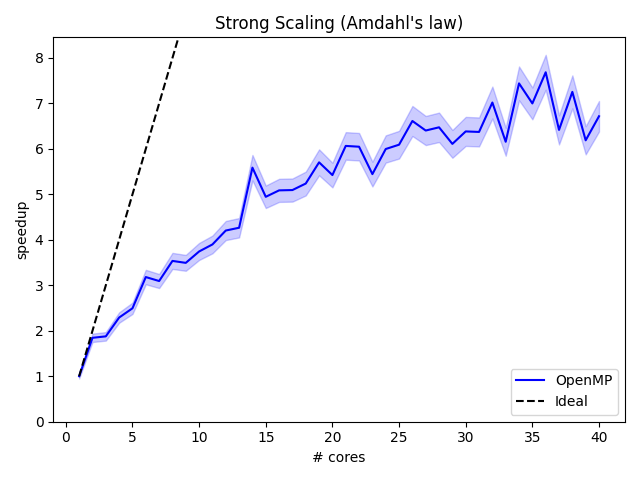
\includegraphics[width=0.75\textwidth]{../plots/strong_scaling.png}
  \caption{Strong scaling of the parallelized implementations}
  \label{fig:strong_scaling}
\end{figure}

\paragraph{Analysis of Figure \ref{fig:strong_scaling}:}
In this graph, we can observe the Strong scaling of the different implementations of the algorithm.
As we can see, the results are in favor of the MPI implementation, due to the diminution in size of the sub parts that each cores will have to sort.

\begin{figure}[H]
  \centering
  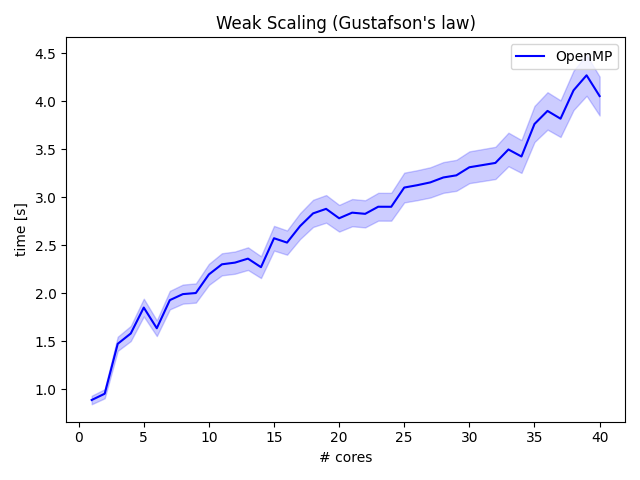
\includegraphics[width=0.75\textwidth]{../plots/weak_scaling.png}
  \caption{Weak scaling of the parallelized implementations}
  \label{fig:weak_scaling}
\end{figure}

\paragraph{Analysis of Figure \ref{fig:weak_scaling}:}
In this graph, we can observe the Weak scaling of the different implementations of the algorithm. For each core, we add a total 
As we can see, the results are in favor of the MPI implementation for a small number of core, but is replaced by the OpenMP implementation for big number of threads, probably due to a better decoupling of concrete work done for each tasks.

\section{Conclusion}

In this report, we have explored the sequential implementation of Merge Sort, followed by two parallel implementations using MPI and OpenMP. We then analyzed their performance through strong and weak scaling experiments. From the results, we can conclude that the MPI implementation provides better performance when dealing with smaller numbers of processes, thanks to better distribution of workload across nodes. However, as the number of threads increases, OpenMP becomes more efficient, likely due to reduced communication overhead and better local memory usage.

Each approach presents trade-offs between ease of implementation, memory management, and scalability. While MPI is suitable for distributed environments with explicit communication control, OpenMP is better in shared-memory systems with simpler thread parallelism.


\end{document}
